%% 
%% Copyright 2007, 2008, 2009 Elsevier Ltd
%% 
%% This file is part of the 'Elsarticle Bundle'.
%% ---------------------------------------------
%% 
%% It may be distributed under the conditions of the LaTeX Project Public
%% License, either version 1.2 of this license or (at your option) any
%% later version.  The latest version of this license is in
%%    http://www.latex-project.org/lppl.txt
%% and version 1.2 or later is part of all distributions of LaTeX
%% version 1999/12/01 or later.
%% 
%% The list of all files belonging to the 'Elsarticle Bundle' is
%% given in the file `manifest.txt'.
%% 

%% Template article for Elsevier's document class `elsarticle'
%% with numbered style bibliographic references
%% SP 2008/03/01

%% Use the option review to obtain double line spacing
%% \documentclass[authoryear,preprint,review,12pt]{elsarticle}

%% Use the options 1p,twocolumn; 3p; 3p,twocolumn; 5p; or 5p,twocolumn
%% for a journal layout:
%% \documentclass[final,1p,times]{elsarticle}
%% \documentclass[final,1p,times,twocolumn]{elsarticle}
%% \documentclass[final,3p,times]{elsarticle}
%% \documentclass[final,3p,times,twocolumn]{elsarticle}
%% \documentclass[final,5p,times]{elsarticle}
%% \documentclass[final,5p,times,twocolumn]{elsarticle}

%% The amsthm package provides extended theorem environments
%% \usepackage{amsthm}

\newif\ifDRAFT
%\DRAFTfalse
\DRAFTtrue

\ifDRAFT
\documentclass[review,number,sort&compress,12pt]{elsarticle}
    %% The lineno packages adds line numbers. Start line numbering with
%% \begin{linenumbers}, end it with \end{linenumbers}. Or switch it on
%% for the whole article with \linenumbers.
%% \usepackage{lineno}
    \usepackage{lineno}
    \newcommand{\picwidth}{0.8\textwidth}
\else 
  \documentclass[final,5p,times]{elsarticle}
    \newcommand{\picwidth}{0.48\textwidth}
\fi

% packages
%\usepackage{fontspec}
%\setmainfont{Gulliver}

\usepackage{amsmath}
\usepackage{amssymb}
\usepackage{bm}
\usepackage{braket}
\usepackage{booktabs}
\usepackage{graphicx}
\usepackage{xcolor}
\usepackage{tikz}
\usetikzlibrary{patterns}
\usepackage{subcaption}
\usepackage{url}
\usepackage{setspace}
\usepackage{diagbox} % generate diagonal divided cell in table
\usepackage{float}
\usepackage{graphicx}
\usepackage{subcaption}
\floatplacement{figure}{H}

\usepackage[linesnumbered,ruled]{algorithm2e}
\usepackage{algpseudocode}
%\usepackage{mathalfa}
%\usepackage{mathrsfs}
\DeclareMathOperator*{\argmin}{argmin}
%\DeclareMathAlphabet{\mathcal}{OT1}{pzc}{m}{bf}
\usepackage[imagesright]{rotating}
%\usepackage{subfigure}
\captionsetup[subfigure]{labelformat=simple,labelsep=colon}
\renewcommand{\thesubfigure}{fig\arabic{subfigure}}



% new commands
\newcommand{\EQ}[1]{Eq.~(\ref{#1})}                
\newcommand{\EQUATION}[1]{Equation~(\ref{eq:#1})} 
\newcommand{\TWOEQS}[2]{Eqs.~(\ref{eq:#1})~and~(\ref{eq:#2})}  
\newcommand{\TWOEQUATIONS}[2]{Equations~(\ref{eq:#1})~and~(\ref{eq:#2})}  
\newcommand{\EQS}[1]{Eqs.~(\ref{#1})}             %-- Eqs. (refeqs)
\newcommand{\EQUATIONS}[1]{Equations~(\ref{#1})}  %-- Eqs. (refeqs)
\newcommand{\FIG}[1]{Fig.~\ref{#1}}               %-- Fig. refig
\newcommand{\FIGURE}[1]{Figure~\ref{#1}}          %-- Figure refig
\newcommand{\TAB}[1]{Table~\ref{#1}}              %-- Table tablref
\newcommand{\SEC}[1]{Section~\ref{#1}}               %-- Eq. (refeq)
\newcommand{\REF}[1]{Ref.~\citen{#1}}               %-- Eq. (refeq)
\newcommand{\BLUE}[1]{\textcolor{blue}{#1}}
\renewcommand{\vec}[1]{\boldsymbol{#1}} %vector is bold italic
\newcommand{\vd}{\bm{\cdot}} % slightly bold vector dot
\newcommand{\grad}{\vec{\nabla}} % gradient
\newcommand{\ud}{\mathop{}\!\mathrm{d}} % upright derivative symbol

\graphicspath{{./figures/}}


\ifDRAFT
\doublespacing
\fi

\journal{Annals of Nuclear Energy}
\usepackage{filecontents,catchfile}

\begin{document}
% \sloppy % prevent words spill into the margin
\begin{frontmatter}

%% Title, authors and addresses

%% use the tnoteref command within \title for footnotes;
%% use the tnotetext command for theassociated footnote;
%% use the fnref command within \author or \address for footnotes;
%% use the fntext command for theassociated footnote;
%% use the corref command within \author for corresponding author footnotes;
%% use the cortext command for theassociated footnote;
%% use the ead command for the email address,
%% and the form \ead[url] for the home page:
%% \title{Title\tnoteref{label1}}
%% \tnotetext[label1]{}
%% \author{Name\corref{cor1}\fnref{label2}}
%% \ead{email address}
%% \ead[url]{home page}
%% \fntext[label2]{}
%% \cortext[cor1]{}
%% \address{Address\fnref{label3}}
%% \fntext[label3]{}

\title{Improvement to the KSU TRIGA reactor}
%% use optional labels to link authors explicitly to addresses:
%% \author[label1,label2]{}
%% \address[label1]{}
%% \address[label2]{}


\author{Jeremy A. Roberts\corref{cor}}
\ead{jaroberts@k-state.edu}
\address{Department of Mechanical and Nuclear Engineering, Kansas State University, Manhattan, KS 66506, USA}
\cortext[cor]{Corresponding author}

\begin{abstract}
	A computational model for the TRIGA reactor at Kansas State University(KSU) has been developed using three 
	different Monte-Carlo simulation tools, namely, MCNP6, Serpent2 and SCALE-6.2.
	
	In addition to the modeling part, all the reactor historical data including the different core configurations, initial fuel loading information and data recorded in the logbooks since 1973 were reviewed and digitized.
	
	Using this model and the reactor data, a depletion sequence has been established throughout the entire 
	operational history to compute the current fuel burnups and also their compositions.\\
	To estimate the current compositions and burnups, two approaches were adopted. The first approach requires running transport calculations only and information about the total energy produced, while the other approach involves depletion calculation, that solves explicitly for the nuclides compositions. The estimated burnups values range up to $\approx$ 49 MWd/kg. The bias between both approaches is calculated and reported in the results along with the values of the computed burnups.
	
	
\end{abstract}

\begin{keyword}
	\texttt{TRIGA}\sep Monte Carlo simulation \sep Burnup 
	\MSC[2010] 00-01\sep  99-00
\end{keyword}
\end{frontmatter}

\linenumbers

\section{Introduction}
Kansas State University has a TRIGA mark II research reactor operating with a maximum power of 1250 kW. Criticality was first achieved in 1962 and since then the facility served for several educational and research purposes.

It is a pool type, light water moderated. The reactor core consists of six concentric rings, (A, B, C, D, E and F). Those rings have 91 locations that could be filled with fuel, control elements and possibly a graphite element.
The fuel is a homogeneous mixture of 20\% enriched uranium, that contributes to 8.5\% of the total weight, and ZrH.

In 1973, the aluminum clad fuel elements  were replaced by fuel elements with a stainless-steel cladding. Those elements had a previous burnup history and the values of their burnups are provided in the original shipment documentation. 
Because those burnups are calculated based on a ring-averaged power estimate, which is not sufficiently accurate, a preliminary study has been conducted to estimate the uncertainty associated with those burnups \cite{gairola2017estimating}.\\ Using those computed uncertainties, an investigatory study was conducted to propagate them to the current compositions uncertainties through a developed surrogate model using Dynamic Mode Decomposition \cite{recent paper}.

This work involves a complete review and improvement of the reactor documentation including the logbooks, the core configurations and the initial fuel loading information.
Also, a fully scripted 3D computational model was developed. Three Monte Carlo simulation tools were used to build the model, namely MCNP6, Serpent 2 and KENO under SCALE-6.2 package.

In order to estimate the current burnups of the fuel elements, the model is used along with the reviewed documentation to establish a depletion sequence starting from the first configuration in 1973 to the current configuration.\\
Two approaches were adopted in this sequence, the first is based on the element-averaged power values and the other involves depletion calculation that solves explicitly for the isotopic concentrations.
The following section gives details about the model development, followed by ????


\section{Model Development}

A fully scripted 3D computational model was developed for the KSU TRIGA reactor. An object-oriented based scripts were written using Python[ref] to develop the model. These scripts contain several classes that are responsible for defining the dimensions, geometry and material library. \\
Also, there is a class for each simulation code involved, i.e MCNP, Serpent and SCALE, that is responsible for writing an input file for the model using the specific code syntax.

For the material library, PyNE \cite{bates2014pyne} was used to define the isotopic compositions of each material included in the model.\\
On top of all those scripts, there is \emph{manager} module that reads the user inputs and accordingly automates writing and running the model input file and also processing the output.\\
The model offers some flexibility in respect to the spatial resolution of the fuel elements since it allows dividing the fuel elements up to 40 axial, 25 radial, and 10 azimuthal segments.\\
Based on the user choice, the model is capable of creating input files for either MCNP6, Serpent-2 or KENO. Also, there is a \emph{calculation mode} option in which the user can choose between running the model with transport calculation only or performing burnup calculation which gives the time dependent compositions.\\
In case of burnup mode, the T6-DEPL sequence is used if SCALE model is selected. In case of MCNP and Serpent, the necessary cards for performing burnup calculation are automatically added. \\
In both modes, the user should specify a value for the power to be used for the fission source estimation in the first option while in the later, it is necessary for computing the flux under which the fuel elements are to be depleted.

Also, in the later option, the user must define the irradiation time which can be one or more intervals and optionally a list of isotopes to be tracked throughout the calculation otherwise there is a list of 62 default isotopes that can be used.

Regarding the geometrical part, the reactor operational manual and the original design drawings were consulted to accurately define the dimensions and the geometrical structure.\\  The model is designed so that it allows for different geometrical levels or extensions. For now, we have two geometrical levels, the first level is to model a single fuel element -fresh or depleted- in a square-pitch cell filled with water as shown in fig.\ref{fig:sigle_element_model}.
 The second level models the full core up to the water surrounding the outer graphite reflector as shown in fig.\ref{fig:full_core_model}.

The first level is set to support some quick and preliminary studies and it has already been used in an exploratory study to build a surrogate model that predicts the isotropic composition of a TRIGA fuel element \cite{abdo2018dds}, \cite{elzohery2018cbg}.\\
Also, this level is used for generating composition table or library as a function of the burnup. The main purpose of this library is to compute the compositions of any fuel element  given its burnup value through linear interpolating.

In order to verify that the three models used the defined dimensions, geometry and materials in a consistent way, we ran two test cases in which a transport calculation is performed and the value of $k_{eff}$ is computed. 
The first test is for a fresh single element and its results are given in table \ref{single_rsults_keff} while the other is for a full core and its results are given in table \ref{full_core_results_keff}.\\
The comparison shows that the three models are consistent if the same cross section library is used. Currently, Serpent model uses only ENDF-7.0 data.\\
%%%%%%%% model figures

\begin{figure}[h]
\centering
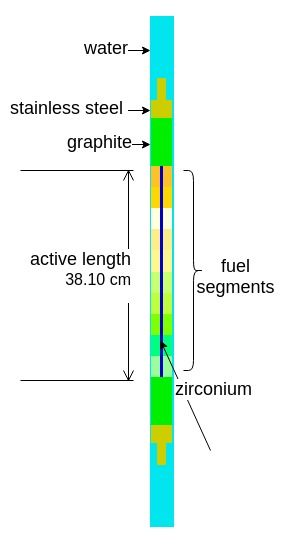
\includegraphics[scale=0.5]{single_element.jpg}\\
\caption{Single element model}
\label{fig:sigle_element_model}
\end{figure}

\begin{figure}[h]
\centering
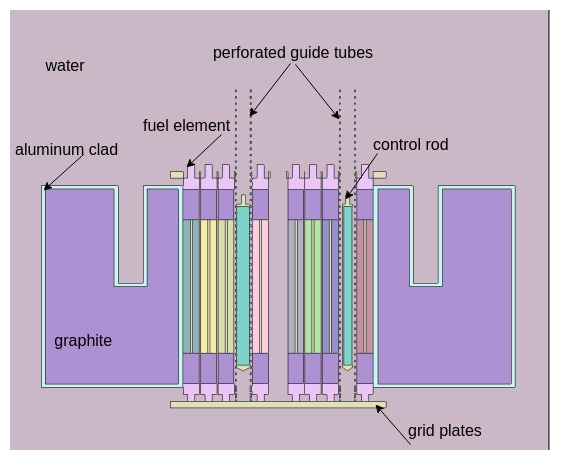
\includegraphics[scale=0.7]{full_core.jpg}\\
\caption{Full core model}
\label{fig:full_core_model}
\end{figure}


%%%%%% keff tables 
\begin{table}[h]
\centering
\caption{Single element results}
\label{single_rsults_keff}
\begin{tabular}{c c c c }
	\hline
	Model & $K_{eff}$ & Thermal Flux ($<$0.625 ev)& Fast Flux\\
	\hline
	KENO (ENDF-7.1)& 1.3203 $\pm$ 0.00023&  $5.267 \times 10^{12}$  & $1.224 \times 10^{13}$ \\
	KENO (ENDF-7.0) & 1.30673 $\pm$ 0.00022&  $5.218 \times 10^{12}$  & $1.219 \times 10^{13}$ \\
	MCNP (ENDF-7.1)& 1.32011 $\pm$ 0.0002 &  $5.284 \times 10^{12}$ & $1.222 \times 10^{13}$ \\
	Serpent (ENDF-7.0) &1.30631 $\pm$ 0.00024&  $5.231 \times 10 ^{12}$  & $1.218 \times 10 ^{13}$\\
\end{tabular}
\end{table}

\begin{table}[h]
\caption{Full core results}
\label{full_core_results_keff}
\begin{tabular}{c c c c }
	\hline
	Model & $K_{eff}$ & Thermal Flux ($<$0.625 ev)& Fast Flux \\
	\hline
	Scale (ENDF-7.1)& 1.03808 $\pm$  0.000362&  $5.409 \times 10^{10}$ & $1.255\times 10^{11}  $ \\
	MCNP (ENDF-7.1)& 1.03734   $\pm$ 0.00022 &  $5.428 \times 10^{10}$ & $1.252\times 10^{11}$\\
	Serpent(ENDF-7.0) & 1.02707  $\pm$  0.00036  & $5.374\times 10^{10}$ & $1.250\times 10^{11}$\\
\end{tabular}
\end{table}

More development and extensions of the model are still undergoing. A graphical user interface(GUI) of the model is supposed to be completed soon which can easily be used by the reactor staff.

Also, the SCALE model can be extended to support some uncertainty and sensitivity studies using TSUNAMI and SAMPLER sequences which will help in identifying the sources of bias in the computed $k_{eff}$.

Currently, the model is being used for core optimization study which takes advantage of the model flexibility that allows for modeling any core arrangement provided by the user with fuel elements compositions corresponding to any burnup values up tp 55 MWd/kg. The model is expected to serve for more studies in the future.

\section{Reactor Data Documentation Review}
The reactor documentations involve the logbooks data, core configurations and the initial fuel loading information.
Each one of those documentations represents an important piece required for estimating the current fuel isotopic compositions.

The logbooks data includes information about the power history recorded since the reactor first operated. The information includes the startup time, operating power, control position, temperature, etc.
A number of undergraduate students at Kansas state university worked on reviewing and digitizing those records and ended up with have one \emph{json} formatted file that contains the data recorded in the logbooks since 1962. 
Figure \ref{fig:core3_power} shows the time dependent power of one of the configurations based on the data recorded in the logbooks

\begin{figure}[h]
\centering
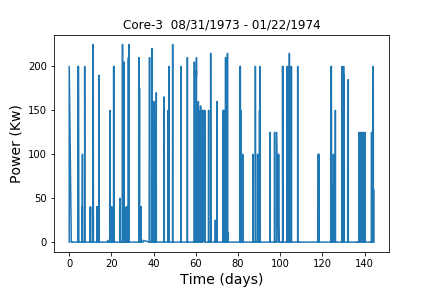
\includegraphics[scale=0.8]{core3.png}\\
\caption{Time dependent power}
\label{fig:core3_power}
\end{figure}


For the core configurations, there are 28 ones, each of which has different core loading pattern. The documentations including those configuration were reviewed and also digitized in a format that can easily be used by the model.
Figure \ref{fig:coreii1_config} shows an example of one of the configurations and also its total energy produced calculated from the data recorded in the logbooks. The numbers inside fuel locations represent the serial number of this fuel element.

\begin{figure}[htp]
\centering
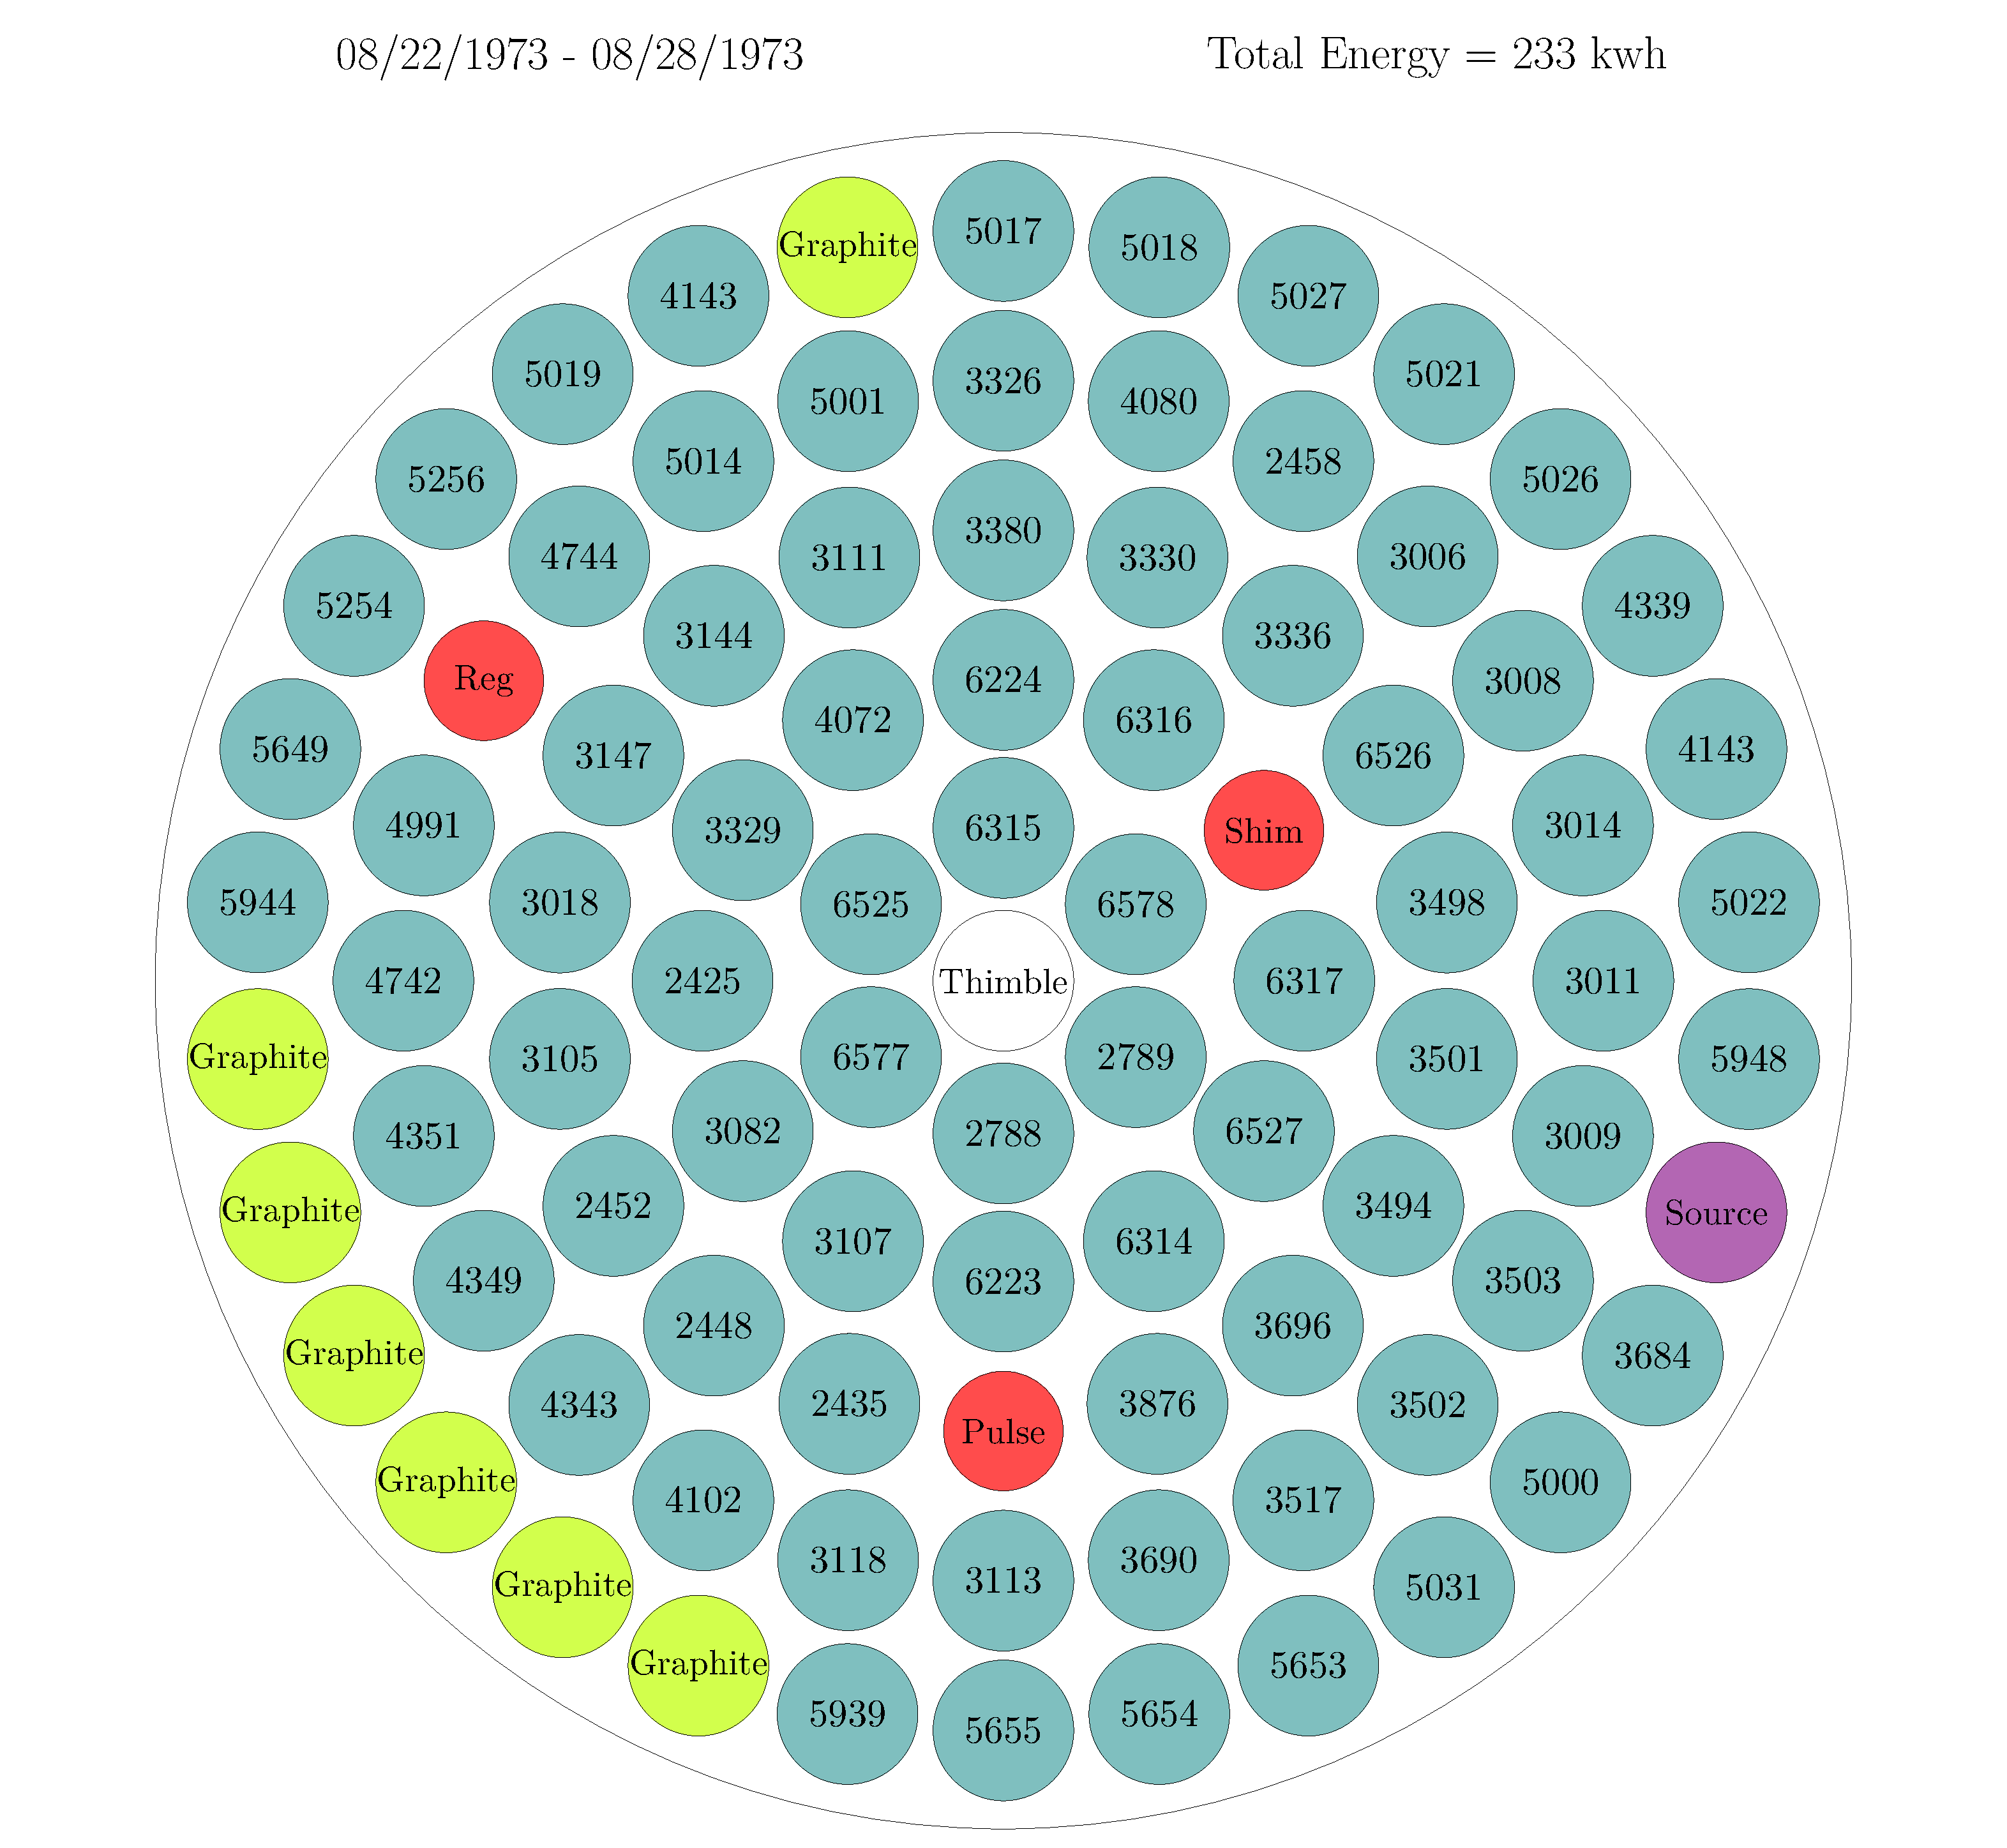
\includegraphics[scale=0.3]{coreii1.pdf}\\
\caption{Core configuration example}
\label{fig:coreii1_config}
\end{figure}

Finally, we reviewed the original shipment documents listing the fuel elements back to 1973 and the ones received in 1985 and 1995. Those documents list every fuel element by its serial number along with its enrichment, uranium weight and burnup value. Also, all the data were compiled and stored in one \emph{json} file.\\
In fact, having all the data in such format was very helpful in establishing and automating the depletion sequence discussed in the next section.


\section{Depletion Sequence}

One major goal of having a computational model for the KSU Triga reactor is to estimate the current composition and burnups of all the fuel elements. To achieve this goal a depletion sequence that marches those compositions forward in time has been established starting form august 1973 to June 2017.\\
A separate class named \emph{DepletionSequence} has been implemented to automate running the sequence. 
Simply, this class loops over all the configurations given by the user, and after running each each configuration, it updates the compositions of the fuel elements to be used as the initial compositions for the next configuration and so on.

As described above, the model can do both transport and burnup calculations. Based on this, two approaches for computing the compositions are implemented.\\
The first approach requires running a transport calculation and in this case, the fuel elements burnups at the end of each configuration can be computed as core-averaged, ring-averaged or element-averaged value based on the computed power peaking factors and the total energy produced in the given configuration. \\
Using this estimated burnup value, the corresponding compositions are
computed by linear interpolating from a pre-generated table that contains the compositions as
a function of the burnup (up to ≈ 55 MWd/kg) and the initial uranium mass.
Those depletion tables are generated using a class named \emph{CompositionGenerator} that is responsible for computing the compositions of any fuel given its information i.e, enrichment, initial uranium mass content, current burnup value, hydrogen to zirconium ratio, etc.

In the second approach, a depletion calculation is performed which solves for the nuclide densities explicitly. For example, in SCALE model, the sequence T6-DEPL is used in which ORIGEN module is invoked to handle nuclide evolution while KENO does the transport calculation.
Also, for MCNP and Serpent the necessary cards for performing depletion calculation are added to both models. In this approach, the compositions are extracted directly from the output files. \\
Once the compositions at the end of each configuration are produced and processed, they are stored in a \emph{json} file which is used to define the initial compositions of the next configuration and so on until the current compositions are computed.\\
To run this depletion sequence, the user should provide a list of names of the text files that contain the different cores arrangements and geometry and for each configuration, the associated power and irradation time have to be specified too. The model is designed so that it has the ability to do a depletion calculation for each configuration given either the total time averaged core power or the time dependent power history of the configuration, which allows for better accuracy.


\section{Burnups estimations}
Based on the depletion sequence discussed above, an estimation of the current burnups is done where the fuel element meat is treated as one axial segment.
In case of the simplified scheme that requires transport calculation, the current burnups of the fuel elements are generated automatically in a text file at the end of the last configuration.\\
However, in the other case where depletion calculations are performed, the energy produced by each fuel element had to be computed after each configuration and then its final accumulated burnup is computed based on the total energy it produced over all the configuration and its initial uranium mass as provided in the original documentation.

The estimated burnups have values that range from about 0.3 to 49 MWd/kg. The burnups computed using SCALE and Serpent for the two approaches are given in table ?? in appendix ??.\\
It was found that the maximum bias between the two approaches is 3.5 \% and 4.1\% for serpent and SCALE respectively, while the maximum bias between SCALE and Serpent for the depletion-calculated burnup is 1.39\%.\\
The results suggest that the simplified scheme can be used as a computationally cheap alternative to the real depletion calculation, which is much more costly, for burnup estimation but to a certain degree of accuracy.

Also, using serpent a comparison study has been done to see the effect of the fuel element spatial resolution on the estimated burnup values. This takes into account the spatial variation of the neutron flux and hence the burnup, so the fuel material was divided into seven equal axial segments and again the burnups were computed using the two aforementioned approaches. 
The maximum bias in the estimated burnup was 0.77\%. the burnups values using seven axial segment are given in table ?? in appendix ??\\ 
\textcolor{red}{(not sure if a study of the bias in keff is needed)}


\section{Conclusion}

\section*{References}

\bibliographystyle{elsarticle-num} 
\bibliography{references}


\end{document}
\endinput
%%
%% End of file `elsarticle-template-num.tex'.
